\documentclass[border=3pt]{standalone}
% Shared TikZ styles for the Ch. 3–8 diagrams (standalone PDFs); extends the Ch. 1 palette (s1_vs_llm_common.tex).
\usepackage[T1]{fontenc}
\usepackage{lmodern}
\usepackage[english]{babel}
\usepackage{amsmath,amssymb}
\usepackage{tikz}
\usetikzlibrary{shapes.geometric,shapes.misc,positioning,fit,arrows.meta,calc,backgrounds,decorations.pathreplacing,patterns}
\definecolor{ioFill}{HTML}{F1F0EC}\definecolor{ioLine}{HTML}{52514E}
\definecolor{modFill}{HTML}{E8F1FB}\definecolor{modLine}{HTML}{2A78D6}
\definecolor{decFill}{HTML}{ECE9F7}\definecolor{decLine}{HTML}{4A3AA7}
\definecolor{postFill}{HTML}{FFF6E0}\definecolor{postLine}{HTML}{EDA100}
\definecolor{okFill}{HTML}{EAF7F1}\definecolor{okLine}{HTML}{1BAF7A}
\definecolor{badFill}{HTML}{FDECEC}\definecolor{badLine}{HTML}{E34948}
\definecolor{nmFill}{HTML}{EFEAF8}\definecolor{nmLine}{HTML}{4A3AA7}
\definecolor{loopRed}{HTML}{E34948}\definecolor{clusterLine}{HTML}{9A9890}\definecolor{ink2}{HTML}{52514E}
\definecolor{orangeA}{HTML}{EB6834}
\tikzset{
  every node/.style={font=\small, align=center},
  io/.style={trapezium, trapezium left angle=72, trapezium right angle=108, trapezium stretches body,
             draw=ioLine, fill=ioFill, thick, inner sep=3pt, minimum height=2.4em},
  model/.style={rectangle, draw=modLine, fill=modFill, very thick, inner sep=4pt, minimum height=2.4em, text width=#1},
  model/.default=3.6cm,
  post/.style={rectangle, draw=postLine, fill=postFill, very thick, inner sep=4pt, minimum height=2.2em, text width=#1},
  post/.default=3.6cm,
  data/.style={cylinder, shape border rotate=90, aspect=0.18, draw=okLine, fill=okFill, very thick, inner sep=3pt, minimum height=2.6em, text width=#1},
  data/.default=2.4cm,
  decision/.style={diamond, aspect=2.1, draw=decLine, fill=decFill, very thick, inner sep=1pt},
  outcome/.style={rounded rectangle, draw=#1, thick, inner sep=4pt, minimum height=2em},
  arrow/.style={-{Latex[length=2mm]}, thick, ioLine},
  dashedarrow/.style={-{Latex[length=2mm]}, thick, ioLine, dashed},
  loop/.style={-{Latex[length=2.4mm]}, line width=1.4pt, loopRed},
  cluster/.style={draw=clusterLine, dashed, rounded corners=3pt, inner sep=7pt},
  clusterlabel/.style={font=\small\bfseries, text=ioLine},
  note/.style={font=\footnotesize, text=ink2},
  tok/.style={rectangle, draw=ioLine, fill=ioFill, thin, inner sep=2pt, minimum height=1.6em, font=\footnotesize},
  vmark/.style={rectangle, draw=orangeA, fill=postFill, thick, inner sep=2pt, minimum height=1.6em, font=\footnotesize\ttfamily},
}

\begin{document}
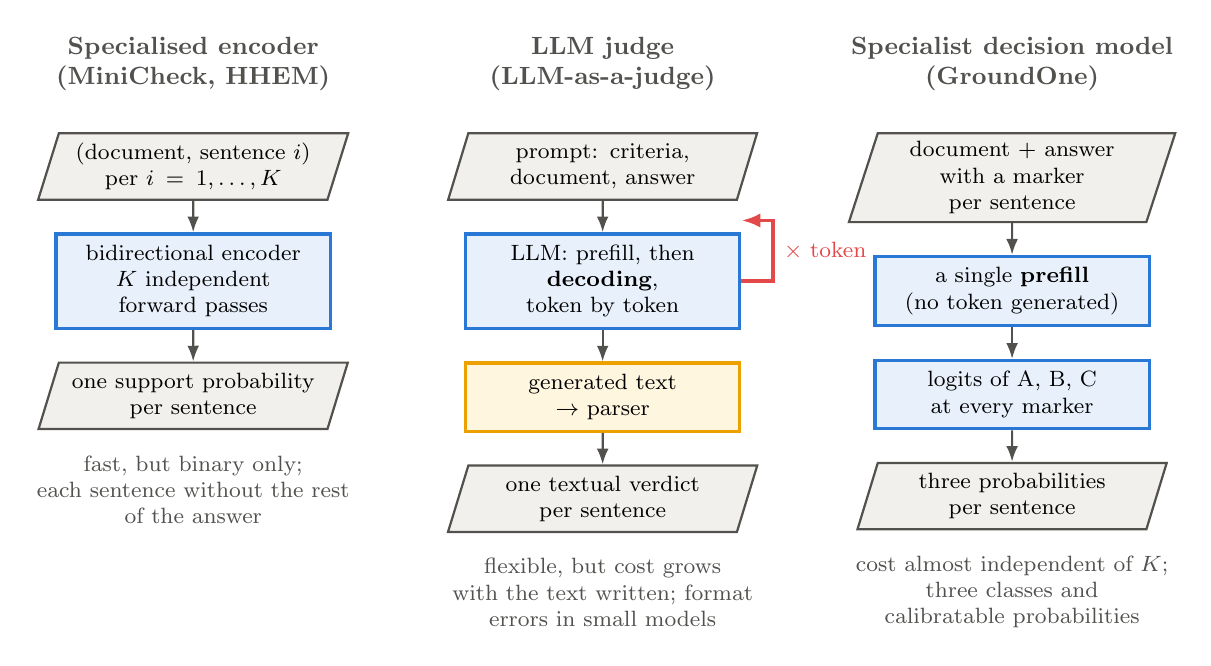
\begin{tikzpicture}[node distance=4mm]
  % column 1: encoder
  \node[clusterlabel] (h1) at (0,0) {Specialised encoder\\(MiniCheck, HHEM)};
  \node[io, text width=3.2cm, below=4mm of h1, font=\footnotesize] (i1) {(document, sentence $i$)\\per $i = 1, \dots, K$};
  \node[model=3.2cm, below=of i1, font=\footnotesize] (m1) {bidirectional encoder\\$K$ independent forward passes};
  \node[io, text width=3.2cm, below=of m1, font=\footnotesize] (o1) {one support probability\\per sentence};
  \node[note, below=2mm of o1] {fast, but binary only;\\each sentence without the rest\\of the answer};
  \draw[arrow] (i1) -- (m1); \draw[arrow] (m1) -- (o1);
  % column 2: judge
  \node[clusterlabel] (h2) at (5.2,0) {LLM judge\\(LLM-as-a-judge)};
  \node[io, text width=3.2cm, below=4mm of h2, font=\footnotesize] (i2) {prompt: criteria,\\document, answer};
  \node[model=3.2cm, below=of i2, font=\footnotesize] (m2) {LLM: prefill, then\\\textbf{decoding},\\token by token};
  \node[post=3.2cm, below=of m2, font=\footnotesize] (p2) {generated text\\$\rightarrow$ parser};
  \node[io, text width=3.2cm, below=of p2, font=\footnotesize] (o2) {one textual verdict\\per sentence};
  \node[note, below=2mm of o2] {flexible, but cost grows\\with the text written; format\\errors in small models};
  \draw[arrow] (i2) -- (m2); \draw[arrow] (m2) -- (p2); \draw[arrow] (p2) -- (o2);
  \draw[loop] (m2.east) -- ++(4mm,0) |- ([yshift=1.5mm]m2.north east) node[pos=0.25, right, note, text=loopRed] {$\times$ token};
  % column 3: system one
  \node[clusterlabel] (h3) at (10.4,0) {Specialist decision model\\(GroundOne)};
  \node[io, text width=3.2cm, below=4mm of h3, font=\footnotesize] (i3) {document + answer\\with a marker per sentence};
  \node[model=3.2cm, below=of i3, font=\footnotesize] (m3) {a single \textbf{prefill}\\(no token generated)};
  \node[model=3.2cm, below=of m3, font=\footnotesize] (r3) {logits of A, B, C\\at every marker};
  \node[io, text width=3.2cm, below=of r3, font=\footnotesize] (o3) {three probabilities\\per sentence};
  \node[note, below=2mm of o3] {cost almost independent of $K$;\\three classes and\\calibratable probabilities};
  \draw[arrow] (i3) -- (m3); \draw[arrow] (m3) -- (r3); \draw[arrow] (r3) -- (o3);
\end{tikzpicture}
\end{document}
